\chapter{\IfLanguageName{dutch}{Stand van zaken}{State of the art}}
\label{ch:stand-van-zaken}
\graphicspath{{../../Images/}} 
% Tip: Begin elk hoofdstuk met een paragraaf inleiding die beschrijft hoe
% dit hoofdstuk past binnen het geheel van de bachelorproef. Geef in het
% bijzonder aan wat de link is met het vorige en volgende hoofdstuk.

% Pas na deze inleidende paragraaf komt de eerste sectiehoofding.

Dit hoofdstuk bevat je literatuurstudie. De inhoud gaat verder op de inleiding, maar zal het onderwerp van de bachelorproef *diepgaand* uitspitten. De bedoeling is dat de lezer na lezing van dit hoofdstuk helemaal op de hoogte is van de huidige stand van zaken (state-of-the-art) in het onderzoeksdomein. Iemand die niet vertrouwd is met het onderwerp, weet nu voldoende om de rest van het verhaal te kunnen volgen, zonder dat die er nog andere informatie moet over opzoeken \autocite{Pollefliet2011}.

Je verwijst bij elke bewering die je doet, vakterm die je introduceert, enz. naar je bronnen. In \LaTeX{} kan dat met het commando \texttt{$\backslash${textcite\{\}}} of \texttt{$\backslash${autocite\{\}}}. Als argument van het commando geef je de ``sleutel'' van een ``record'' in een bibliografische databank in het Bib\LaTeX{}-formaat (een tekstbestand). Als je expliciet naar de auteur verwijst in de zin, gebruik je \texttt{$\backslash${}textcite\{\}}.
Soms wil je de auteur niet expliciet vernoemen, dan gebruik je \texttt{$\backslash${}autocite\{\}}. In de volgende paragraaf een voorbeeld van elk.

\textcite{Knuth1998} schreef een van de standaardwerken over sorteer- en zoekalgoritmen. Experten zijn het erover eens dat cloud computing een interessante opportuniteit vormen, zowel voor gebruikers als voor dienstverleners op vlak van informatietechnologie~\autocite{Creeger2009}.
\newpage
\section{Versiebeheer}
\subsection{Inleiding}
\label{sec:vb_inleiding}
Versiebeheer is een belangrijk concept binnen softwareontwikkeling. Zo waren er in totaal 100 miljoen projecten op het populaire versiebeheer platform GitHub (in 2018) \autocite{Git2018}. GitHub (sinds 2018 overgenomen door Microsoft) is niet de enige speler op de markt. Zo is er ook nog Code Commit van Amazon en GitLab. Veel bedrijven en oplossingen spelen dus in op de behoefte voor een duidelijk en efficiënt versiebeheer systeem. Toch kan men stilstaan bij de vraag: Welke behoefte lossen deze systemen op?

Stel volgende scenario voor: Alice en Bob zijn aangenomen om te werken voor Bedrijf X. Hun eerste taak is een website ontwikkelen. Ze leggen samen alle vereisten vast, bespreken de verschillende technologieën en gaan aan de slag. Op het einde van de eerste dag hebben ze elk een verschillende pagina gemaakt en deze willen ze graag met elkaar delen.Dit kan door bijvoorbeeld via mail de bestanden door te sturen. Een andere mogelijkheid is de bestanden via fysieke hardware zoals een USB-Stick aan elkaar te geven. Het nadeel is dat de code op twee verschillende plaatsen verspreid zit. Als Bob de code die hij heeft geschreven kwijt raken, dan zal deze opnieuw moet worden geschreven. Om dit probleem te voorkomen kan men het project op een centrale server opslaan. Bob en Alice zullen hun veranderingen opslaan op deze centrale server. Zo hebben ze altijd toegang tot elkaars werk. 

Deze manier van werken heeft zijn eigen nadelen. Alice kan per ongeluk een bestand overschrijven of een stuk code verwijderen. Tenzij men back-ups heeft is het originele bestand verloren. Om dit probleem te omzeilen wordt er gebruik gemaakt van het concept van \textbf{versies}. Elke aanpassing die er gemaakt wordt resulteert in een nieuwe versie van het project. Men kan altijd terugkeren naar een eerdere versie. Als Alice dus het stukje code verwijdert in versie 15 kan men terug naar versie 14.

\textcite{Loeliger2009} stelt dat een versiebeheersysteem een middel is om verschillende versie van code te beheren en bijhouden. De auteur onderscheid volgende drie eigenschappen waaraan dergelijke systemen voldoen:

\begin{itemize}
	\item Er wordt gebruik gemaakt van een centraal Archief. Binnen dit archief worden alle versies van het project bewaard en bijgewerkt.
	\item Het centraal archief geeft toegang tot eerdere versies van het project.
	\item Alle veranderingen die worden aangebracht aan het archief worden genoteerd in een centraal logboek.
\end{itemize}

Versiebeheer is geen nieuw concept. Er zijn zoals eerder aangehaald verschillende software oplossingen beschikbaar. Toch zijn er volgens \textcite{Chacon2014} drie grote categorieën (zie \ref{fig:TypesVCS} voor een grafische weergave):

\begin{itemize}
	\item Lokale versiebeheersystemen: het centraal archief waar de veranderingen in worden bewaard staat op een lokale computer. Het grootste voordeel is dat een lokaal systeem zeer makkelijk te onderhouden is. Het is eveneens eenvoudig op te stellen. Toch is het niet geschikt om bestanden met elkaar te  delen of samen aan bestanden te werken. Een gekend voorbeeld is RCS (Revision Control System) - zie \ref{sec:RCS} -. \\
	
	\item CVCS: Om samen te kunnen werken aan dezelfde bestanden kan een CVCS (Centralised Version Control System) worden gebruikt. In plaats van het archief lokaal bij te houden wordt er gebruik gemaakt van een centrale server. Bestanden worden vervolgens lokaal gekopieerd. Als er veranderingen worden aangebracht zullen deze worden doorgestuurd naar de server.Doordat men verplicht is om de bestanden op een centrale plaats af te halen, kan men deze afschermen. Zo kan men toegang beperken tot enkel de nodige bestanden per gebruiker. \\
	
Een neveneffect van alles centraal te beheren is het zogenaamde \textit{single point of failure(SPOF)} probleem. Een SPOF is een onderdeel van een systeem dat mocht het uitvallen heel het systeem tot een halt roept. Met andere woorden valt het centraal archief weg heeft niemand nog toegang tot het project. Een mogelijke oplossing voor dit probleem is redundantie. Dit betekent het aanbieden van kopieën. \autocite{Sun2007}\\

	\item DVCS: Om het SPOF probleem te voorkomen kan men kopieën maken van het centraal archief. Deze kopieën kunnen vervolgens worden verspreid over verschillende computers. Dit is het uitgangspunt van DVCS (Distributed version control System). Elke gebruiker heeft een lokale kopie van de centrale server. De veranderingen aan de bestanden worden eerst aangebracht in het lokaal archief en vervolgens gesynchroniseerd met de centrale variant.\\

Mocht het centraal aanspreekpunt niet beschikbaar zijn is dit geen probleem. Elke gebruiker heeft immers een volledige back-up van het volledige project. In theorie kan de gebruiker zelfs optreden als nieuwe centrale server.
\end{itemize}


\begin{figure}[h!]
	\centering
	\begin{subfigure}[b]{.5\textwidth}
	\centering
		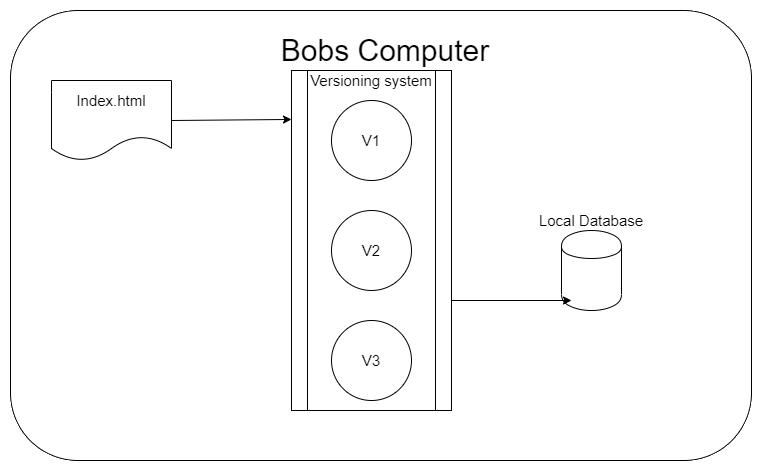
\includegraphics[scale=.3]{LVCS.png}
		\caption[Overzicht structuur Lokale VCS]{Overzicht van de structuur van een Lokale VCS.}
	\end{subfigure}%
	\begin{subfigure}[b]{.5\textwidth}
	\centering
		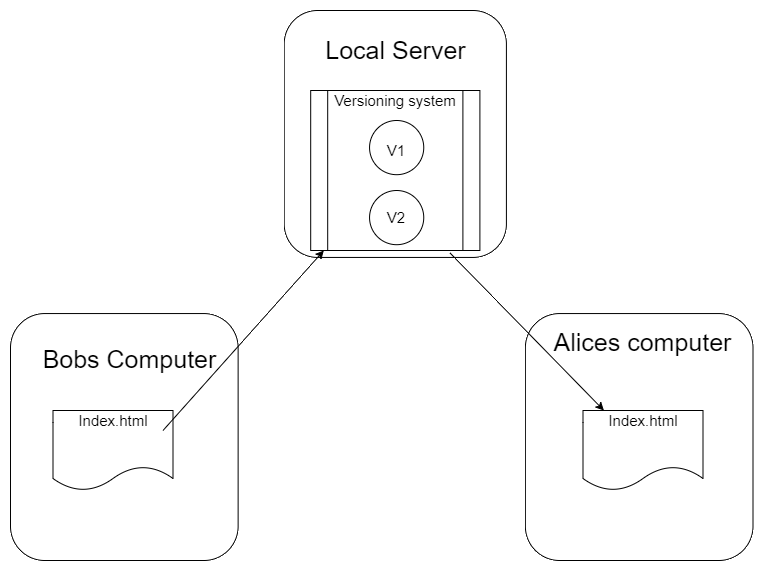
\includegraphics[scale=.3]{CVCS.png}
			\caption[Overzicht structuur CVCS]{Overzicht van de structuur van een CVCS.}
	\end{subfigure}%
	\hfill
	\begin{subfigure}{.5\textwidth}
		\centering
		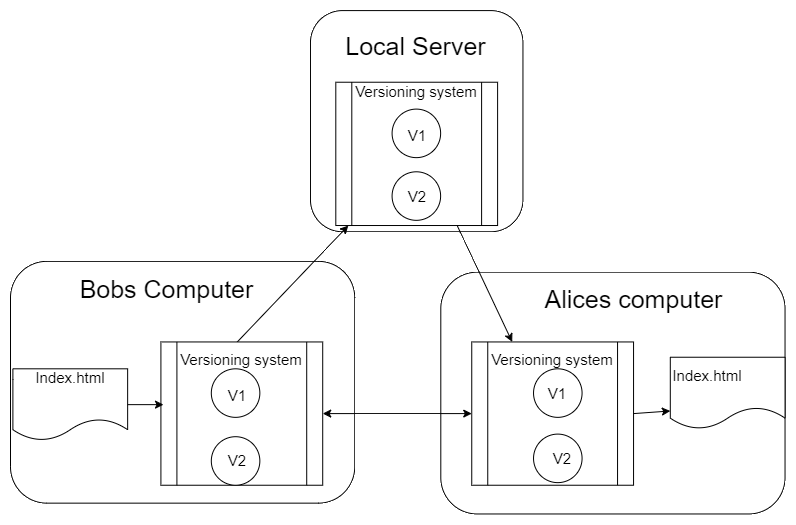
\includegraphics[scale=0.3]{DVCS.png}
	\caption[Overzicht structuur DVCS]{Overzicht van de structuur van een DVCS.}
	\end{subfigure}
	
	\caption[Overzicht types VCS]{Overzicht van de drie types van VCS zoals aangegeven door \textcite{Chacon2014}.}
	\label{fig:TypesVCS}
\end{figure}

	
\subsection{RCS}
\label{sec:RCS}


RCS \textit{(Revision Control System)} is een lokaal versiebeheer systeem. Het is vastgelegd in een artikel geschreven door \textcite{Tichy85rcs}. Het is opgenomen binnen het GNU project -Een open source besturingssysteem \footnote{GNU is veel meer dan enkel open source. Het GNU project is sterk verbonden met de ideologie en organisatie van de free software foundation (FSF). Meer informatie omtrent deze organisatie en beweging is te vinden op: \url{https://www.fsf.org/}}- die het gebruikte als vervanging voor het CSSC Systeem \autocite{GNUCSSC}.\\

CSSC is een systeem gebaseerd op SCCS (Source code control system) dat ontwerpen is voor UNIX systemen. SCCS is in opdracht van Bell Labs ontwikkeld door \textcite{Rochkind1975}. Er is ook nog tal van andere software ontwikkeld voordat RCS op de markt kwam. Zo was er ook nog CA-Panvalet een gepatenteerde oplossing voor Mainframe computers. Toch is het interessanter om RCS in detail te bekijken. Veel van de concepten waar het gebruik van maakt zijn ook aanwezig in moderne systemen (zoals GIT). De manier waarop het is opgebouwd kadert eveneens binnen de visie van deze bachelorproef. Het is open source en wordt nog steeds op vrijwillige basis onderhouden. De onderstaande uitleg over de werking van de software is gebaseerd op \textcite{Tichy85rcs}.\\

Een eerste concept binnen de software is dat van een boomstructuur -denk hier aan een stamboom. Volgens \textcite{Lievens2019}, is een boom een collectie van \textbf{toppen} \textit{(in het engels ook wel Nodes genoemd)}. Deze toppen hebben een hiërarchische verband.Zo bestaat er bijvoorbeeld een kind-ouder verband. Er zijn twee bijzondere toppen in een boom:

\begin{itemize}
	\item De wortel(\textit{root}): Deze top ligt helemaal aan het begin van de boom. Alle andere toppen zijn afstammelingen van deze top. Het heeft aldus geen ouders.
	\item Een blad(\textit{leaf}): Deze top heeft geen kinderen. In tegenstelling tot een wortel kunnen er meerdere bladeren aanwezig zijn.
\end{itemize}

Alle andere toppen worden intermediair genoemd. Elke top heeft mogelijks een aantal kinderen. Elk van deze kinderen is op zijn beurt de wortel voor een nieuwe deelboom. Het concept van \textbf{diepte} is ook belangrijk. De diepte van de wortel is nul ($d$=1) en elk kind heeft als diepte: 

\begin{equation}
	d_{kind} = d_{ouder} + 1
\end{equation}

Al deze concepten worden ook nog eens grafisch verduidelijkt in de grafiek \ref{fig:tree}.

\begin{figure}[h!]
\centering
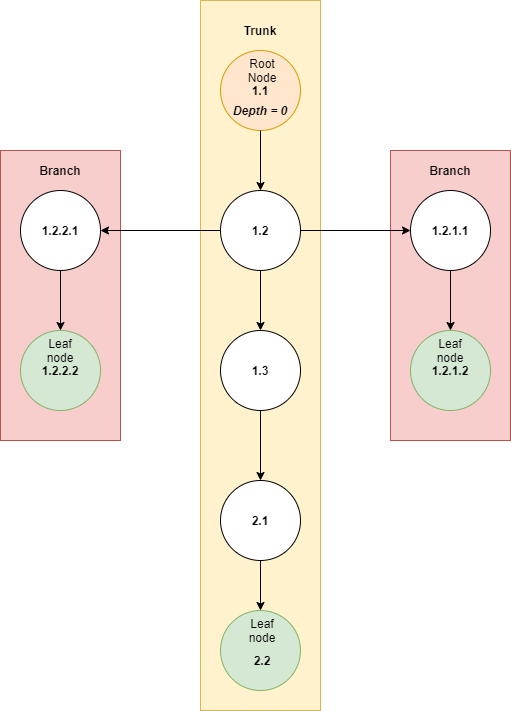
\includegraphics[scale=0.5]{tree1.png}
\label{fig:tree}
\caption[Overzicht concepten boomstructuur]{Een overzicht van alle concepten binnen een boomstructuur waar RCS van gebruik maakt.}
\end{figure}

Er kan gebruik gemaakt worden van een boomstructuur om de onderlinge relaties tussen de versie weer te geven. Stel: Bob en Alice zijn bezig aan de hoofdpagina. Bob maakt een initiële versie van de pagina. Vervolgens wilt hij die graag delen met Alice. Hiervoor gebruikt hij het commando om een nieuwe versie aan te maken\footnote{\Verb+ci homepage.html+}. Dit commando wordt \textbf{inchecken} genoemd. Binnen GIT is dit vergelijkbaar met het commando \textit{git push}. Aangezien dit de eerste versie is kan men dit vergelijken met het aanmaken van een wortel. Volgende versies worden kinderen van de vorige versie. Zo wordt versie 1.4 kind van versie 1.3. Inchecken gaat niet alleen onze boomstructuur aanmaken maar ook de extensie \textit{.v} toevoegen (\verb+homepage.html.v+). Het originele bestand wordt ook verwijderd\\

Het bestand krijgt ook een \textbf{versie nummer}. Dit versienummer heeft de vorm: $x_1.x_2$. $x_1$ (ook wel \textit{release} genoemd) staat voor een grote verandering. Bijvoorbeeld het in productie nemen van een nieuwe versie.$x_2$ (\textit{level}) staat voor een kleinere verandering. Een andere manier om $x_2$ te bekijken is de diepte met als wortel de laatste release ($x_1$). 1.1 is het versienummer van de wortel die Bob heeft aangemaakt. 1.4 is het derde kind van de wortel.Elke check-in zal het level ($x_2$) met één verhogen. Het release nummer ($x_1$) wordt manueel verhoogd door middel van de \textit{-r} optie bij check-in \footnote{\Verb+ci -r2 homepage.html+}. Bij branches is er ook nog spraken van $x_3$ en $x_4$ zie \ref{par:branches}. Deze manier van versies te bestempelen wordt nog steeds gebruikt. Het is echter niet de enige manier. \textit{Semantic versioning} is een gekend alternatief. Het concept van versienummers bestaat in Git onder de vorm van \textit{tags} (\ref{sec:GIT}).\\

Er is nu een bestand onder de vorm \verb+homepage.html.v+. Hoe kan Alice nu dit bestand aanpassen en een nieuwe versie publiceren? Alice gaat het bestand moeten \textbf{uitchecken}.Dit kan ze doen door middel van het commando \verb+co+ en de naam van het bestand \footnote{(\Verb+co homepage.html+)} . Het uitchecken is aldus het verkrijgen van een specifieke versie uit het archief. Als er geen specifieke versie wordt meegegeven wordt de laatste versie opgehaald. Om een specifieke versie op te halen kan er gebruik gemaakt worden van de optie -r  \footnote{(\Verb+co -r1.1 homepage.html+)} . Alice heeft nu een kopie van het originele bestand gekregen. Merk op dat in tegenstelling tot inchecken ons archief niet wordt verwijderd. Vervolgens kan ze in deze lokale kopie wijzigingen aanbrengen. Tot slot wordt het bestand weer aan het lokaal archief toegevoegd door middel van inchecken. Het equivalent van \verb+co+ binnen git is \verb+git pull+.\\

\begin{wrapfigure}{r}{0.5\textwidth}
\label{fig:deltas}
\begin{center}
  	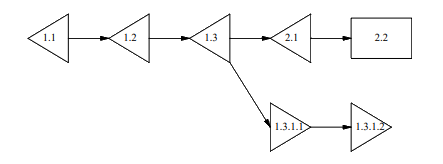
\includegraphics[scale=0.6]{deltas.png}
\end{center}
\caption[Voorbeeld van deltas.]{Een voorbeeld van deltas.De Trunk bevat een series van achterwaardse deltas terwijl alle branches enkel voorwaardse deltas bevatten. Grafiek afkomstig uit \textcite{Tichy85rcs}}
\end{wrapfigure}

Hoe worden de verschillen tussen de versies bijgehouden in ons lokaal archief. Een mogelijke oplossing zou zijn om alle versies van het bestand afzonderlijk bij te houden. Dit vraagt veel opslagruimte. RCS gebruikt voor dit probleem het concept van \textbf{deltas}. Een delta houd bij welke regels veranderd zijn ten opzichte van de vorige versie. Doordat de delta enkel de relevante lijnen gaat bijhouden wordt de opslag beperkt \footnote{De delta wordt opgebouwd aan de hand van het GNU commando diff \url{https://www.gnu.org/software/diffutils/}}. Er zijn twee types van deltas: \textbf{voorwaardse deltas} en \textbf{achterwaardse deltas}. Bij het inchecken van een nieuwe versie zal de vorige versie worden vervangen door een achterwaardse delta. Zit men momenteel op versie 1.3 en  vraagt men versie 1.2 dan zal de achterwaardse delta van versie 1.2 worden toegepast op versie 1.3. Voorwaardse deltas komen aanbod in het gedeelte over branching (\ref{par:branches}). Het concept van deltas wordt nog eens verduidelijkt door een voorbeeld in de appendix -zie \ref{ch:voorbeeld-rcs}-.\\

Inchecken en uitchecken ligt aan de basis van het archiefsysteem. Toch is er nog een probleem aanwezig binnen deze manier van werken. Stel dat Alice en Bob gelijktijdig wijzigingen aanbrengen aan een bestand. Ze willen dit bestand elk afzonderlijk publiceren.  Hierdoor ontstaan er twee versies die afstammen van één gezamenlijke versie. De boomstructuur wordt in twee gesplitst. Dit is niet mogelijk aangezien een versie altijd uniek moet zijn. Hoe kan men verzekeren dat elke versie slechts één kind heeft (op dezelfde branch)? Dit probleem wordt opgelost door \textbf{sloten}(engels=lock).Dit concept geeft gebruikers de mogelijkheid om een versie te  versleutelen. Terwijl een versie versleuteld is kan niemand anders wijzigingen aanbrengen. Andere gebruikers kunnen deze nog bekijken. Op het moment dat Bob zijn versie gaat uitchecken kan hij deze versleutelen (door middel van de \textit{-l} optie bij het co commando). Hierdoor kan Alice geen nieuwe versie meer aanmaken tot Bob zijn wijzigingen heeft doorgevoerd. Met andere woorden zolang bob het slot niet vrijgeeft kunnen er geen nieuwe versies worden aangemaakt\footnote{In sommige gevallen kan het slot ook worden 'geforceerd' mocht Bob bijvoorbeeld ziek vallen}. Deze manier van werken heeft een zichtbaar nadeel. Alice is verplicht om te wachten op Bob zijn nieuwe versie alvorens ze veranderingen kan maken. Git gebruikt het concept van sloten niet. Daar maakt men gebruik van \textbf{merges} om dit zelfde probleem aan te pakken \ref{sec:GIT}.

\section{branches}
\label{par:branches}
In de vorige paragraaf wordt aangehaald, dat elke versie exact één kind heeft. Dit is echter niet de volledige realiteit. Er is eveneens het concept van \textbf{takken} (eng: branches. Net zoals stambomen kunnen vertakken, kan dit ook in het archief.De originele boom wordt de \textbf{trunk} genoemd. \textcite{Tichy85rcs} geeft enkele redenen om dit toe te passen:

\begin{itemize}
\item Doorvoeren van veranderingen in oude versies. Hierbij wordt volgend voorbeeld gegeven: Een bedrijf gebruikt een oude versie van een software product. Deze software is ontwikkeld met behulp van RCS. Het bedrijf ontdekt een fout in de vorige versie en vraagt een rechtzetting. Aangezien er al nieuwere versies zijn kan men niet eenvoudig een nieuwe versie gaan publiceren. Hiervoor kan men aldus een vertakking maken en de wijzigingen daarop aanbrengen.
\item Verschillende implementatie versies. Stel dat een ontwikkelaar een andere manier van werken wilt gaan verkennen. Mocht dit op de hoofdboom (\textit{trunk})gebeuren zou men het risico lopen dat de software onstabiel wordt. Het zou dus meer afgeschermd zijn mocht de ontwikkelaar werken op een afzonderlijke tak.
\end{itemize}

De tweede reden vertoond veel gelijkenissen met 
\subsubsection{Opmerkingen}
In het originele artikel wordt de klemtoon gelegd op het onderling delen van de verschillende versies. Hierdoor kan men de indruk krijgen dat er een centrale server betrokken is. Dit is niet het geval. De software is ontworpen om op één besturingssysteem uitgevoerd te worden. Volgens \textcite{Debian2020} is GNU aangezien het gebaseerd is op UNIX een \textit{multi-user os}. Dat wil zeggen dat meerdere gebruikers het systeem tezelfdertijd kunnen gebruiken door middel van een terminal connectie. Hierdoor kan men onderling de bestanden delen ondanks dat men niet gaat werken in een CVCS -zie \ref{sec:CVCS}-.

\subsection{CVCS}
\label{sec:CVCS}

\subsection{GIT}
\label{sec:GIT}
